Consider the gridworld and value function in the figure below.
Using your knowledge of the transition dynamics and the values (numbers in each grid cell), write down the policy corresponding to taking the greedy action with respect to the values in each state.
Create a grid with the same dimension as the figure and draw an arrow in each square denoting the greedy action.

The details of the environment are as follows. The cells of the grid correspond to the states of the environment. At each cell, four actions are possible: north, south, east, and west, which deterministically 
cause the agent to move one cell in the respective direction on the grid. Actions that would take the agent off the grid leave its location unchanged, but also result in a reward of -1.
Other actions result in a reward of 0, except those that move the agent out of the special states A and B. From state A, all four actions yield a reward of +10 and take the agent to A'. From state B, all actions yield a reward of +5 and take the agent to B'.
\begin{figure}[h!]
  \center
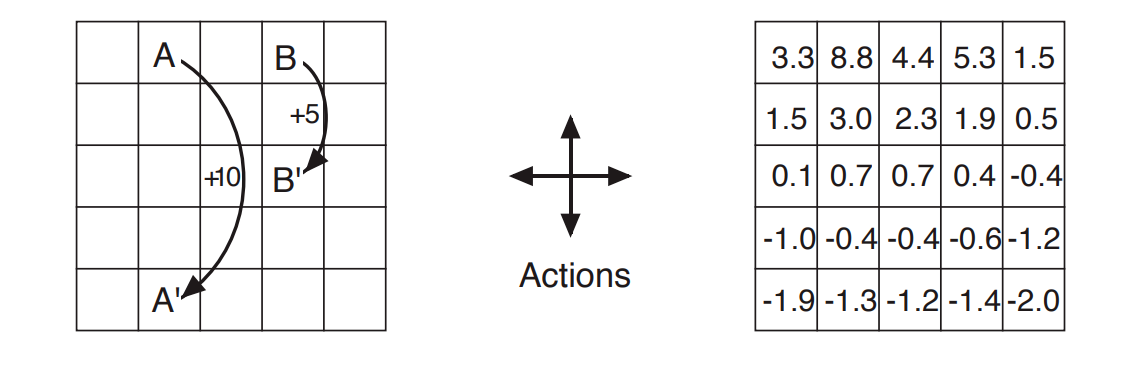
\includegraphics[width=0.9\linewidth]{figures/figure_3dot2.png}
\end{figure}

\bigspace